\documentclass[10pt]{article}
\usepackage{icmlko}

\icmlmeta{IP 파운데이션 월드모델}{230}{계열이 둘이라는 것도 재야 한다}{노트 229가 남긴 유일한 길은 셋째 계열이었다. 상관 행렬을 재니 계열이 둘인 것은 맞고, 셋째는 없다}

\begin{document}

\twocolumn[
\icmlheader

\begin{abstract}
노트 229가 ``F23 이 유일한 무선택 형태''임을 보이고 남긴 유일한 열린
길이 \textbf{셋째 계열}이었다. 그런데 ``계열이 둘''은 내가 선형·트리로
\emph{이름 붙인} 것이지 잰 것이 아니었다. 쟀다. 여섯 정식화의 유보 예측
상관 행렬을 만들고 이름 없이 묶으니 \textbf{2 묶음이 정확히
\{F21 · F6 · F9 · F19\} 대 \{F18 · F8\} 로 갈린다} --- 선형 대 트리다.
\textbf{계열 안 상관 중앙 0.975 · 계열 간 0.820 · 차 $+$0.155} 다.
\textbf{계열이 둘이라는 것이 이제 잰 것이다.} 그리고 셋째 후보 둘이 다
탈락한다. \textbf{F9 는 셋째 계열이 아니다} --- 제곱오차가 아니라 짝 순위
우도로 맞추는데 \textbf{F6 와 상관이 0.999} 다. \textbf{목적함수를 바꿔도
예측이 안 바뀐다.} 남는 후보는 F19(무리 쌓기)뿐이다 --- 선형 무리 안에서
유일하게 떨어져 있고(F21 과 0.868, 다른 둘은 0.976 · 0.975) 3 묶음으로
자르면 혼자 나온다. 그런데 \textbf{섞을 값이 없다} --- 셋을 1/3 씩 섞으면
$-$0.0078($t{=}-2.53$)이고 무게를 0.2 로 줄여도 $-$0.0041($t{=}-2.12$)로
유의하게 손해다. \textbf{떨어져 있는 것과 값이 있는 것은 다르다.} 여섯을
``F21 로부터의 거리''와 ``판''으로 놓으면 그림이 하나로 정리된다 ---
\textbf{선형 무리 안에서는 멀수록 약하고}(F6 0.024/$+$.4250 · F9
0.025/$+$.4236 · F19 0.132/$+$.4089), \textbf{멀면서 센 것은 트리
하나뿐이다}(F18 0.171/$+$.4408). \textbf{포트폴리오 안에 셋째 방향은
없다.} F23 의 천장은 두 대표가 정하고, 그것을 넓히려면 새 계열을
\emph{만들어야} 한다 --- 고르는 문제가 아니다.
\end{abstract}
]

\begin{figure*}[t]
\centering
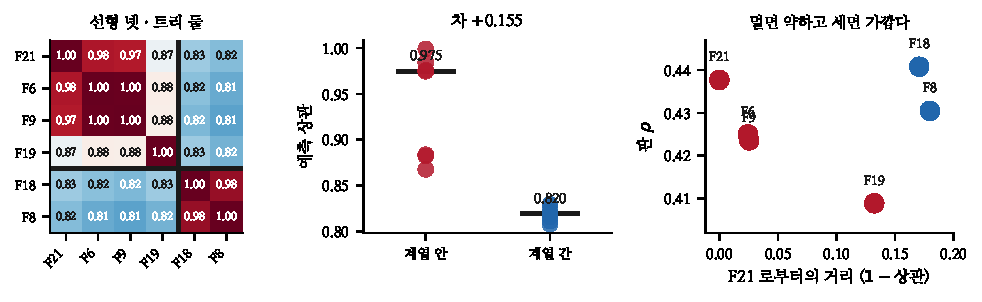
\includegraphics[width=\textwidth]{figs/twofamilies.pdf}
\caption{왼쪽 --- 상관 행렬이 선형 넷 · 트리 둘로 갈린다. 가운데 ---
계열 안과 계열 간의 차. 오른쪽 --- 멀면 약하고 세면 가깝다.}
\end{figure*}

\section{계열이 둘인 것은 맞다}

\begin{table}[t]
\centering\tsize
\caption{유보 예측의 스피어만(표본 수 가중).}
\begin{tabular}{lrrrrrr}
\toprule
& F21 & F6 & F9 & F19 & F18 & F8 \\
\midrule
F21 & --- & .976 & .975 & .868 & .829 & .820 \\
F6 & & --- & \textbf{.999} & .884 & .822 & .812 \\
F9 & & & --- & .883 & .819 & .808 \\
F19 & & & & --- & .830 & .816 \\
F18 & & & & & --- & \textbf{.984} \\
\bottomrule
\end{tabular}
\end{table}

\claimx{\textbf{이름 없이 묶으면 2 묶음이 정확히 선형 넷 대 트리 둘이다.}
계열 안 상관 중앙 0.975 · 계열 간 0.820 · 차 $+$0.155.}{\textbf{노트
225$\sim$229 가 ``계열''이라고 부른 것이 이제 잰 것이다} --- 그전까지는
내가 모형 종류를 보고 붙인 이름이었고, 노트 225의 순위 역전이 그 이름과
맞아떨어진 것이 근거의 전부였다.}

\section{셋째 후보 둘이 탈락한다}

\claimx{\textbf{F9 는 셋째 계열이 아니다} --- 제곱오차가 아니라 짝 순위
우도로 맞추는데 \textbf{F6 와 상관이 0.999} 다.}{\textbf{목적함수를 바꿔도
예측이 안 바뀐다.} 노트 229가 ``F9 는 목적함수가 다르므로 따로 세워 볼
값이 있다''고 적었는데 \textbf{값이 없다} --- 그리고 그것을 판이 아니라
상관으로 먼저 알 수 있었다.}

\begin{table}[t]
\centering\tsize
\caption{F19 를 섞으면. F23 대비 짝 붓스트랩 500 회.}
\begin{tabular}{lrrr}
\toprule
& 판 & 차 & $t$ \\
\midrule
\textbf{F21$+$F18 (F23)} & \textbf{.4534} & --- & --- \\
$+$F19 (1/3 씩) & .4455 & $-$.0078 & $-$2.53 \\
$+$F19 (.4/.4/.2) & .4493 & $-$.0041 & $-$2.12 \\
F21$+$F19 & .4330 & $-$.0205 & $-$3.72 \\
F19 혼자 & .4089 & $-$.0443 & $-$5.36 \\
\bottomrule
\end{tabular}
\end{table}

\claimx{\textbf{F19 는 선형 무리 안에서 유일하게 떨어져 있는데}(F21 과
0.868, 다른 둘은 0.976 · 0.975) \textbf{섞을 값이 없다} --- 무게를 0.2 로
줄여도 $-$0.0041($t{=}-2.12$)이다.}{\textbf{떨어져 있는 것과 값이 있는
것은 다르다.} 노트 227이 ``상관이 낮으면 섞인다''를 근거로 F23 을
세웠는데, \textbf{낮은 상관은 필요조건이지 충분조건이 아니다.}}

\section{멀면 약하고 세면 가깝다}

\begin{table}[t]
\centering\tsize
\caption{F21 로부터의 거리($1-$상관)와 판.}
\begin{tabular}{lrrl}
\toprule
& 거리 & 판 & \\
\midrule
F21 & .000 & .4377 & 선형 \\
F6 & .024 & .4250 & 선형 \\
F9 & .025 & .4236 & 선형 \\
\textbf{F19} & \textbf{.132} & \textbf{.4089} & 선형 \\
\textbf{F18} & \textbf{.171} & \textbf{.4408} & \textbf{트리} \\
F8 & .180 & .4305 & 트리 \\
\bottomrule
\end{tabular}
\end{table}

\claimx{\textbf{선형 무리 안에서는 멀수록 약하다}(0.024 $\to$ $+$.4250 ·
0.025 $\to$ $+$.4236 · 0.132 $\to$ $+$.4089). \textbf{멀면서 센 것은
트리 하나뿐이다}(0.171 $\to$ $+$.4408).}{\textbf{그래서 포트폴리오 안에
셋째 방향이 없다.} 섞어서 얻으려면 \emph{멀고도 센} 것이 필요한데,
있는 것은 멀고 약한 것(F19)과 가깝고 약한 것(F6 · F9)뿐이다.}

\claimx{\textbf{F23 의 천장은 두 대표가 정한다.} 넓히려면 새 계열을
\emph{만들어야} 하고 그것은 고르는 문제가 아니다.}{노트 229가 ``F2 결합
잠재''를 후보로 적었는데 적합 한 번이 110초라 이 사이클에서 못 쟀다 ---
\textbf{다음 사이클의 첫 칸이고, 재기 전에 상관부터 보면 값이 있는지 미리
안다.}}

\begin{table}[t]
\centering\tsize
\caption{남은 것.}
\begin{tabular}{ll}
\toprule
\textbf{F2 결합 잠재} & 유일하게 안 잰 후보 --- 상관부터 \\
\textbf{새 계열} & 멀고도 센 것을 만들 수 있나 \\
F1 & 이 축 판에서 nan --- 왜인지 안 봤다 \\
\bottomrule
\end{tabular}
\end{table}

셋째 줄이 값싸고 이 노트가 만든 빚이다. \textbf{F1 프로크루스테스가 이
축 판에서 판 nan 을 냈는데 그냥 넘어갔다.} F1 은 노트 5$\sim$124 의 옛
파이프라인이고 포트폴리오의 기준선이다 --- \textbf{기준선이 안 돌아가는
것을 모르고 있었다는 뜻이다.} 노트 187의 제일 값싼 검사(``판이 안 움직이면
모형에 안 닿은 것'')의 사촌이다: \textbf{판이 nan 이면 그 정식화는 이
판에서 죽어 있고, 죽은 줄 모르면 포트폴리오가 여섯이 아니라 다섯이다.}

\end{document}
